\documentclass{article}
\usepackage{ProfLycee}
\useproflyclib{ecritures}
\usepackage{tikz}
\begin{document}

Un industriel doit fabriquer une boîte fermée de volume $1\,\text{L}$, soit $1\,\text{dm}^3$, ayant la forme d'un pavé de hauteur $h$ dont la base est un carré de côté $x$. L'unité de longueur est le $\text{dm}$.

\begin{enumerate}
  \item Justifier que $h = \dfrac{1}{x^2}$.
  
  \item En déduire que l'aire totale des faces du pavé est $S = 2x^2 + \dfrac{4}{x}$.
  
  \item Montrer que pour $x > 0$, on a $S'(x) = \dfrac{4(x-1)(x^2+x+1)}{x^2}$.
  
  \item En déduire les variations de $S$.
  
  \item Donner les dimensions de la boîte d'aire minimale.
\end{enumerate}


\begin{enumerate}
  \item Le volume de la boîte est $1\,\text{dm}^3$ donc $\mathcal{V}=x \times x \times h = 1$ d'où $h = \dfrac{1}{x^2}$.
    
    \item L'aire totale des faces du pavé est $$S(x) = \mathcal{A}_{\text{base}}\times 2+\mathcal{A}_{\text{latérale}}\times 4 = 2x^2 + 4xh = 2x^2 + 4x\times \dfrac{1}{x^2} = 2x^2 + \dfrac{4}{x}$$
    
    \item $S$ est dérivable sur $\IntervalleOO{0}{+\infty}$ et $S'(x) = 4x - \dfrac{4}{x^2} = \dfrac{4x^3-4}{x^2}$.
    
    De plus: $4(x-1)(x^2+x+1) = 4(x^3+x^2+x-x^2-x-1) = 4(x^3-1) = 4x^2-4$.

    On en déduit que pour tout $x \in \IntervalleOO{0}{+\infty}$ $$S'(x) = \dfrac{4(x-1)(x^2+x+1)}{x^2}$$

    \item On étudie le signe de $x^2+x+1$. $\Delta = 1-4 = -3 < 0$ donc $x^2+x+1 > 0$ pour tout $x \in \R$.
    
    $S'(x)$ est donc du signe de $x-1$.

    On a donc le tableau de variations suivant:

    \begin{center}
    \begin{tikzpicture}
    \tkzTabInit{$x$ / 1 , $S'(x)$ / 1, $S(x)$ / 1.5}{$0$, $1$, $+\infty$}
    \tkzTabLine{, -, z, +,}
    \tkzTabVar{+/ $~$, -/ $6$, +/ $~$}
    \end{tikzpicture}
    \end{center}

    \item La boîte d'aire minimale est celle pour laquelle $S$ est minimale, c'est-à-dire pour $x=1$. C'est un cube de côté $1$.
\end{enumerate}


\end{document}